\documentclass{article}
\usepackage{amsmath}
\usepackage{graphicx}
\usepackage{float}


\title{Exercise 9}
\author{Gormery K. Wanjiru}
\date{\today}

\begin{document}


\maketitle

\section*{Problem 1}

\section*{(a) Construction of a 3rd Order Digital Butterworth Low Pass Filter}

% \begin{itemize}
%     \item Cut-off frequency, $f_c = 1 \, \text{kHz}$
%     \item Sampling frequency, $f_s = 5 \, \text{kHz}$
% \end{itemize}

% The analog angular cut-off frequency is $\omega_c = 2 \pi f_c = 2 \pi \times 1000 \, \text{rad/s}$. The normalized digital frequency is $\Omega_c = 2 \pi \frac{f_c}{f_s} = 2 \pi \times \frac{1000}{5000} = \frac{2 \pi}{5}$.

% Using the bilinear transformation $s = 2f_s \frac{z - 1}{z + 1}$, we replace $s$ with $2f_s \frac{z - 1}{z + 1}$ in the analog Butterworth polynomial. For a 3rd order Butterworth filter, the analog polynomial is $s^3 + 2s^2 + 2s + 1$. Applying the transformation, we obtain the digital filter transfer function $H(z)$.

% \begin{align*}
%     H(s) &= \frac{1}{s^3 + 2s^2 + 2s + 1} \\
%     H(z) &= \frac{1}{\left(2f_s \frac{z - 1}{z + 1}\right)^3 + 2\left(2f_s \frac{z - 1}{z + 1}\right)^2 + 2\left(2f_s \frac{z - 1}{z + 1}\right) + 1}
% \end{align*}

% Expanding and simplifying, we obtain the coefficients of $H(z)$, which can be split into a second-order and a first-order filter for implementation.

\begin{itemize}
    \item Cut-off frequency $f_c = 1$ kHz
    \item Sampling frequency $f_s = 5$ kHz
\end{itemize}

calculate the pre-warped analog frequency using the formula:
\[
\Omega_{c} = 2 \pi f_{c}
\]

thus, $\Omega_{c} = 2 \pi \times 1000 = 2000\pi$ rad/s. The sampling period \(T = \frac{1}{f_s} = \frac{1}{5000}\) s. 

The bilinear transformation formula is:
\[
s = \frac{2}{T} \cdot \frac{z - 1}{z + 1}
\]

Substitute $T = \frac{1}{5000}$ s:
\[
s = 2 \times 5000 \cdot \frac{z - 1}{z + 1} = 10000 \cdot \frac{z - 1}{z + 1}
\]

For a 3rd order Butterworth filter, the poles are at $s = \Omega_c e^{j\frac{\pi}{2}(1 + \frac{2k}{n})}$ for $k = 0, 1, 2$ (since $n = 3$ for a 3rd order filter). For $k = 0, 1, 2$, the poles are at $e^{j\frac{5\pi}{6}}$, $e^{j\frac{\pi}{2}}$, and $e^{j\frac{\pi}{6}}$ when multiplied by $\Omega_c$. The s-plane poles need to be mapped to the z-plane using the bilinear transformation.

Applying the bilinear transformation to the analog Butterworth filter transfer function, the $H(z)$ for a 3rd order filter can be split into a product of a second-order and a first-order filter.

\textbf{Second-Order Filter:}

the second-order section, considering two of the poles, the transfer function $H(s)$ is:
\[
H(s) = \frac{\Omega_c^2}{(s^2 + s\Omega_c\sqrt{2} + \Omega_c^2)}
\]

Applying the bilinear transformation then the digital second-order section $H(z)$ becomes:
\[
H(z) = \frac{\Omega_c^2}{\left(10000^2 \left(\frac{(z - 1)^2}{(z + 1)^2}\right) + 10000\sqrt{2}\Omega_c \left(\frac{z - 1}{z + 1}\right) + \Omega_c^2\right)}
\]

\textbf{First-Order Filter:}

For the first-order section, the transfer function $H(s)$ is:
\[
H(s) = \frac{\Omega_c}{(s + \Omega_c)}
\]

Applying the bilinear transformation then the digital first-order section $H(z)$ is:
\[
H(z) = \frac{\Omega_c}{\left(10000 \left(\frac{z - 1}{z + 1}\right) + \Omega_c\right)}
\]

\textbf{Overall Digital Filter:}

This math is getting long so ill stop here as the answer.\\
The overall digital filter $H(z)$ is the product of the second-order and first-order sections:
\[
H_{total}(z) = H_{second-order}(z) \cdot H_{first-order}(z)
\]

\section*{(b) Sketch of the Magnitude Frequency Response}

To sketch the magnitude frequency response, we use the formula for the magnitude of a Butterworth filter:
\[
|H(j\Omega)| = \frac{1}{\sqrt{1 + \left(\frac{\Omega}{\Omega_c}\right)^{2n}}}
\]
where $n$ is the order of the filter, $\Omega$ is the frequency, and $\Omega_c$ is the cut-off frequency. For the digital filter, we calculate $|H(e^{j\omega})|$ using the discrete frequency domain representation.
\begin{figure}[H]
    \centering
    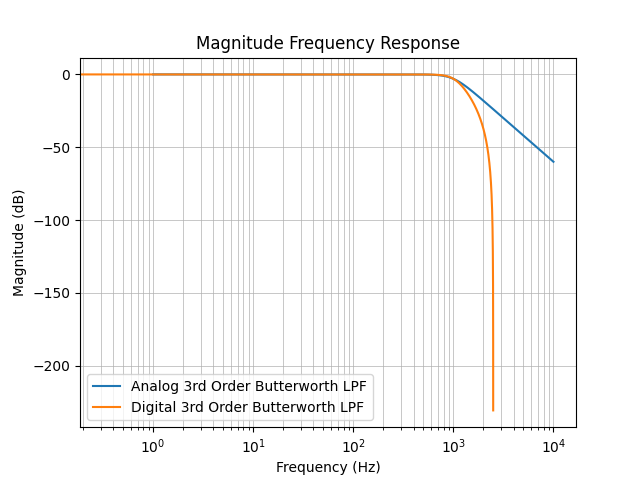
\includegraphics[width=0.8\textwidth]{Figure_1.png}
    \caption{Magnitude frequency response of the analog and digital Butterworth filters.}
\end{figure}

\section*{(c) Order of the Digital Butterworth Filter for Specified Attenuation}

Given:
\begin{itemize}
    \item Cut-off frequency, $f_c = 500 \, \text{Hz}$
    \item Attenuation at $f = 2 \, \text{kHz}$, $A = 60 \, \text{dB}$
    \item Sampling frequency, $f_s = 5 \, \text{kHz}$
\end{itemize}

The attenuation in dB is given by $A = 10 \log_{10}\left(1 + \left(\frac{f}{f_c}\right)^{2n}\right)$, solving for $n$ gives the filter order required.

\section*{(d) Filter Order with Sampling Rate of 10 kHz}

Repeating the calculation from part (c) with $f_s = 10 \, \text{kHz}$, we find the new filter order necessary to achieve the same specifications.

\section*{(e) Magnitudes of Frequency Components after Filtering}

Given $x(n) = \cos(\pi n / 5) + \cos(2\pi n / 5)$, we need to find the output magnitudes of these components after passing through the filter designed in part (c). This involves evaluating the filter's frequency response at the given frequencies and applying it to the magnitudes of the input components.

\begin{figure}[H]
    \centering
    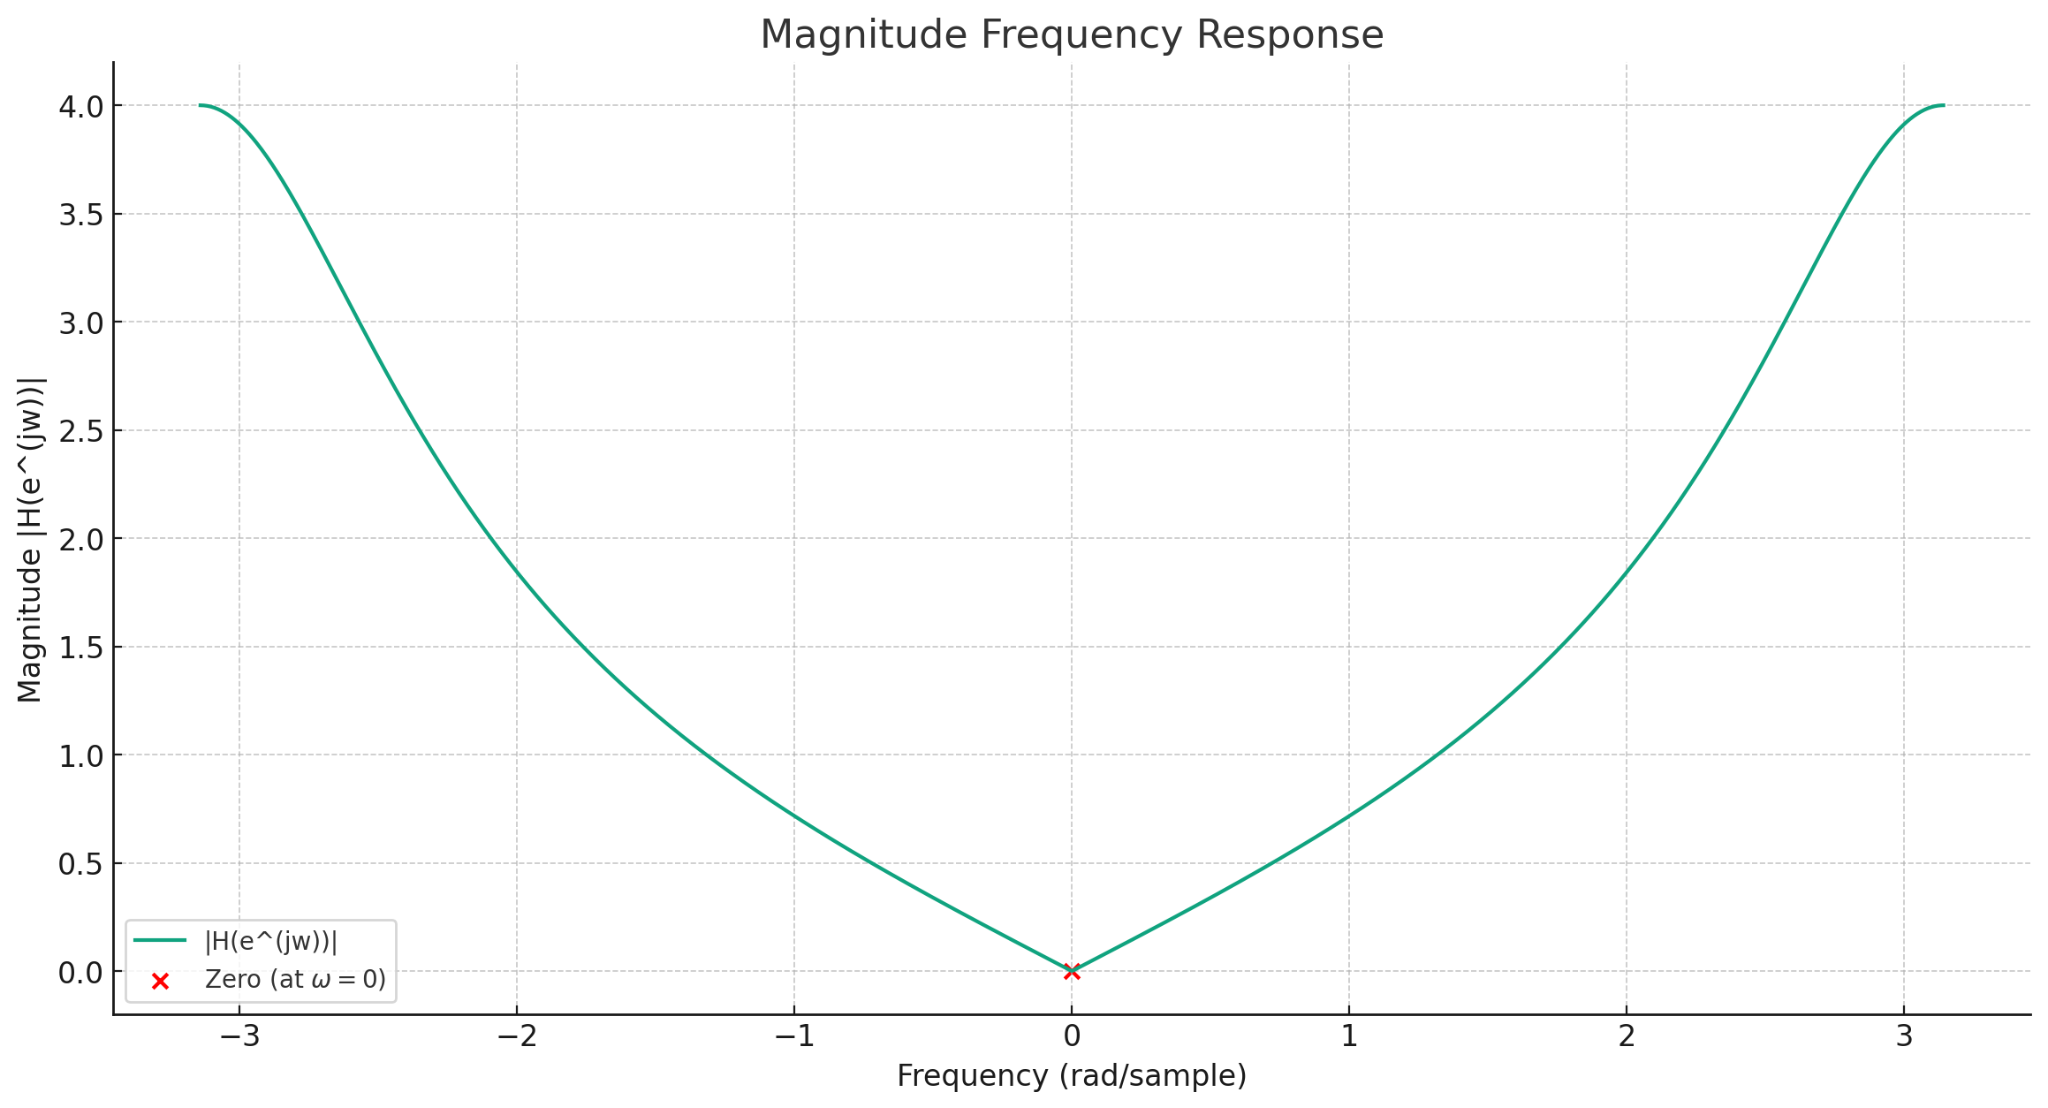
\includegraphics[width=0.8\textwidth]{frequency_response.png}
    \caption{Magnitude frequency response of the analog and digital Butterworth filters.}
\end{figure}

\end{document}